% =====================================================================
%  Mini Proposal Hackathon Deeptech 2026: Indonesia Chip Hackathon Challenge
%  SeBatt: Secure Battery Identity Chip (Tim NaS, Universitas Gadjah Mada)
%  Kompilasi: latexmk -pdf main.tex  (atau pdflatex main.tex dua kali)
%  Format wajib: A4, Arial 11 pt, spasi 1,15, Bagian A-B maks. 5 halaman,
%  Bagian B 200-1.000 kata, CV maks. 1 halaman per anggota.
% =====================================================================
\documentclass[11pt,a4paper]{article}

% ---------- Tata letak & huruf ----------
\usepackage[a4paper,margin=2.54cm]{geometry}
\usepackage[T1]{fontenc}
\usepackage[utf8]{inputenc}
\usepackage[scaled=0.92]{helvet}        % pengganti Arial untuk pdflatex
\renewcommand{\familydefault}{\sfdefault}
\usepackage{microtype}
\usepackage{setspace}
\setstretch{1.15}
\setlength{\parindent}{0pt}
\setlength{\parskip}{6pt}

\usepackage[table]{xcolor}
\usepackage{graphicx}
\graphicspath{{figures/}}
\usepackage{tabularx}
\usepackage{array}
\usepackage{enumitem}
\usepackage{titlesec}
\usepackage{caption}
\usepackage{float}
\usepackage{fancyhdr}
\usepackage{tikz}
\usetikzlibrary{positioning,arrows.meta,fit,backgrounds}
\usepackage[hidelinks]{hyperref}
\usepackage{xurl}
\urlstyle{same}
\frenchspacing
\hypersetup{
  pdftitle={SeBatt: Secure Battery Identity Chip - Mini Proposal},
  pdfauthor={Tim NaS, Universitas Gadjah Mada},
  pdfsubject={Hackathon Deeptech 2026: Indonesia Chip Hackathon Challenge 2026},
}

% ---------- Warna (mengikuti template) ----------
\definecolor{hdrgray}{HTML}{F2F2F2}
\definecolor{subtle}{HTML}{6B7280}

% ---------- Judul bagian ----------
\titleformat{\section}{\large\bfseries\raggedright}{}{0em}{}
\titleformat{\subsection}{\normalsize\bfseries\raggedright}{}{0em}{}
\titlespacing*{\section}{0pt}{14pt}{4pt}
\titlespacing*{\subsection}{0pt}{10pt}{2pt}

\newcommand{\todo}[1]{\textcolor{red}{\textbf{[#1]}}}
\newcommand{\hdr}[1]{\cellcolor{hdrgray}\textbf{#1}}
\newcolumntype{L}[1]{>{\raggedright\arraybackslash}p{#1}}
\newcolumntype{Y}{>{\raggedright\arraybackslash}X}

\setlist[enumerate]{leftmargin=1.6em,itemsep=2pt,topsep=2pt}
\newcommand{\rujuk}[1]{[\ref{#1}]}   % sitasi bernomor ke daftar B7
\captionsetup{font=small,labelfont=bf,labelsep=period}
\renewcommand{\figurename}{Gambar}
\renewcommand{\tablename}{Tabel}
\renewcommand{\arraystretch}{1.25}

\pagestyle{fancy}
\fancyhf{}
\renewcommand{\headrulewidth}{0pt}
\fancyfoot[C]{\footnotesize\color{subtle}ChipHack26 --- NaS --- Mini Proposal \quad|\quad \thepage}

% =====================================================================
\begin{document}

\begin{center}
  {\Large\bfseries Mini Proposal}\\[2pt]
  {\large Hackathon Deeptech 2026: Indonesia Chip Hackathon Challenge 2026}\\[2pt]
  Tema: ``Designing Chips for Real-World Impact''
\end{center}

% ---------------------------------------------------------------------
\section{A. Identitas Tim}

\begin{tabularx}{\linewidth}{|L{3.4cm}|Y|}
  \hline
  \hdr{Item} & \hdr{Isian} \\ \hline
  Judul usulan & SeBatt - Secure Battery Identity Chip : Perancangan IP Keamanan Berbasis PUF dan HMAC-SHA-256 untuk Autentikasi Baterai Kendaraan Listrik \\ \hline
  Nama tim & NaS \\ \hline
  Tema & Internet of Things \\ \hline
  Ketua tim & Guntur Sulistyo \\ \hline
\end{tabularx}

\vspace{8pt}
{\small
\begin{tabularx}{\linewidth}{|c|L{3.9cm}|L{3.3cm}|Y|L{3.2cm}|}
  \hline
  \hdr{No} & \hdr{Nama} & \hdr{NIM} & \hdr{Program studi/Divisi Instansi/Divisi Perusahaan} & \hdr{Perguruan tinggi/ Instansi/Perusahaan} \\ \hline
  1 & Guntur Sulistyo & 22/505305/TK/55288 & Teknik Elektro & Universitas Gadjah Mada \\ \hline
  2 & Dimas Eryan Ahnaf Fahrezi & 23/518972/TK/57204 & Teknik Elektro & Universitas Gadjah Mada \\ \hline
  3 & Muhammad Muqtada Alhaddad & 22/500341/TK/54841 & Teknologi Informasi & Universitas Gadjah Mada \\ \hline
\end{tabularx}
}

% ---------------------------------------------------------------------
\section{B. Deskripsi Usulan Produk}

\subsection{B1. Ringkasan}

SeBatt adalah \textit{Secure Battery Identity Chip} yang ditanam pada paket baterai kendaraan listrik untuk membuktikan keaslian baterai dan keaslian riwayat tegangan yang direkam selama pemakaian. Chip membaca tegangan paket melalui ADC secara berkala, lalu menggunakan \textit{Physical Unclonable Function} (PUF) dan HMAC-SHA-256 untuk menandatangani identitas dan setiap sampel bernomor urut. Kunci tidak disimpan di memori chip, melainkan diturunkan ulang dari PUF setiap kali dibutuhkan. Dengan demikian, pemalsuan identitas, manipulasi riwayat tegangan, dan serangan \textit{replay} dapat dideteksi oleh stasiun.

\subsection{B2. Masalah dan Pengguna Sasaran}

Sistem penukaran baterai kendaraan listrik perlu memastikan dua hal pada setiap baterai yang diterima, yaitu identitas yang dapat dipercaya dan data kondisi yang jujur. Nomor seri dan kode QR dapat disalin. Data tegangan, jumlah siklus, dan riwayat pemakaian dikirim oleh firmware \textit{Battery Management System} (BMS), sehingga dapat diubah sebelum sampai ke stasiun, termasuk pada baterai yang identitasnya asli. Stasiun hanya dapat mengukur tegangan sesaat ketika baterai ditukar, sehingga riwayat selama pemakaian bergantung sepenuhnya pada laporan BMS. Kondisi tersebut dapat menyebabkan kerugian bagi operator, menyulitkan pemeriksaan riwayat baterai, dan meningkatkan risiko penggunaan baterai yang tidak memenuhi standar keselamatan.

Skala masalah tersebut tumbuh bersama jumlah kendaraan listrik roda dua, yang menurut Rencana Usaha Penyediaan Tenaga Listrik (RUPTL) PLN 2025--2034 \rujuk{ref:ruptl} mencapai sekitar 168 ribu unit di Indonesia pada akhir 2024.

Pengguna sasaran SeBatt meliputi operator stasiun penukaran baterai, produsen baterai dan BMS, penyedia layanan sewa baterai, serta lembaga tepercaya yang mengelola basis data identitas baterai.

\subsection{B3. Solusi yang Diusulkan}

Chip SeBatt memanfaatkan \textit{Ring-Oscillator} PUF \rujuk{ref:suh}, \rujuk{ref:maes} untuk memperoleh karakteristik unik perangkat, lalu menghitung respons HMAC-SHA-256 terhadap \textit{nonce}, yaitu angka acak sekali pakai yang diberikan stasiun melalui basis data identitas.

Selain identitas, chip mengambil sampel tegangan paket secara berkala melalui ADC dengan antarmuka I2C (ADS1115 pada prototipe). Setiap sampel diberi nomor urut dari penghitung di dalam IP yang hanya dapat bertambah, lalu ditandatangani HMAC bersama ID baterai. Saat penukaran, stasiun meminta riwayat sampel dan respons atas \textit{nonce} yang memuat nomor urut terakhir, lalu basis data menghitung ulang setiap HMAC. Sampel yang diubah, dihapus, atau disisipkan oleh firmware BMS maupun di jalur komunikasi menghasilkan tanda tangan atau urutan yang tidak cocok sehingga ditolak. Pada produk, chip berkomunikasi melalui bus CAN yang umum digunakan BMS.

Pada \textit{proof of concept}, IP ditulis dalam Verilog/SystemVerilog standar tanpa IP vendor maupun prosesor lunak, sehingga dapat dipindahkan ke FPGA yang disediakan panitia. Kontroler I2C untuk ADC, FSM autentikasi, dan antarmuka UART seluruhnya berupa logika RTL. PC yang terhubung melalui UART, sebagai pengganti bus CAN, menjalankan Python sebagai emulator stasiun dan basis data untuk mengirim \textit{nonce}, memverifikasi respons, serta mencatat hasil autentikasi.

\begin{figure}[H]
  \centering
  \resizebox{\linewidth}{!}{%
  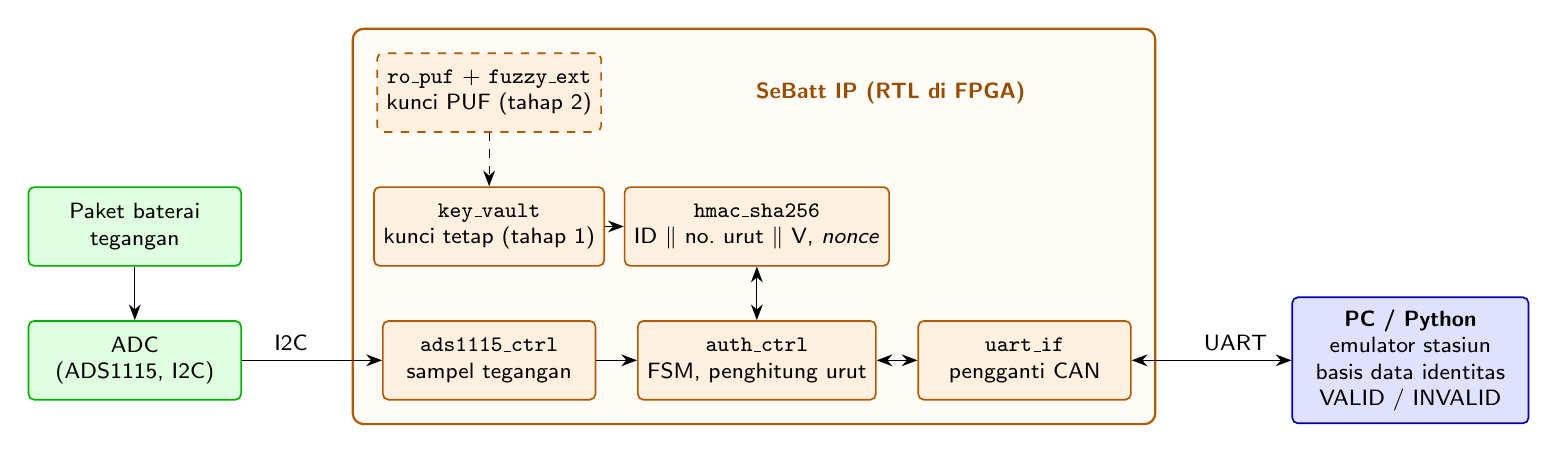
\begin{tikzpicture}[
      font=\footnotesize, >={Stealth[length=2mm]},
      blk/.style={draw=#1!70!black, fill=#1!12, rounded corners=2pt, align=center,
                  minimum width=27mm, minimum height=10mm, line width=0.6pt},
      ip/.style={blk=orange},
      stage2/.style={ip, dashed}]
    % sensor
    \node[blk=green] (bat) at (-0.9,1.7) {Paket baterai\\tegangan};
    \node[blk=green] (adc) at (-0.9,0)   {ADC\\(ADS1115, I2C)};
    % IP di FPGA
    \node[stage2] (puf)  at (3.6,3.4) {\texttt{ro\_puf} + \texttt{fuzzy\_ext}\\kunci PUF (tahap 2)};
    \node[ip]     (key)  at (3.6,1.7) {\texttt{key\_vault}\\kunci tetap (tahap 1)};
    \node[ip]     (adcif) at (3.6,0)  {\texttt{ads1115\_ctrl}\\sampel tegangan};
    \node[ip]     (hmac) at (7.0,1.7) {\texttt{hmac\_sha256}\\ID $\|$ no.~urut $\|$ V, \textit{nonce}};
    \node[ip]     (fsm)  at (7.0,0)   {\texttt{auth\_ctrl}\\FSM, penghitung urut};
    \node[ip]     (uart) at (10.4,0)  {\texttt{uart\_if}\\pengganti CAN};
    \node[font=\footnotesize\bfseries, text=orange!60!black] (lbl) at (8.7,3.4) {SeBatt IP (RTL di FPGA)};
    \begin{scope}[on background layer]
      \node[draw=orange!70!black, fill=orange!3, rounded corners=4pt, line width=0.8pt,
            inner sep=3mm, fit=(puf)(adcif)(uart)(lbl)] (fpga) {};
    \end{scope}
    % stasiun
    \node[blk=blue, minimum width=30mm, minimum height=16mm] (pc) at (15.3,0)
      {\textbf{PC / Python}\\emulator stasiun\\basis data identitas\\VALID / INVALID};
    % panah
    \draw[->] (bat) -- (adc);
    \draw[->] (adc) -- node[above, pos=0.35]{I2C} (adcif);
    \draw[->] (adcif) -- (fsm);
    \draw[->, dashed] (puf) -- (key);
    \draw[->] (key) -- (hmac);
    \draw[<->] (fsm) -- (hmac);
    \draw[<->] (fsm) -- (uart);
    \draw[<->] (uart) -- node[above, pos=0.65]{UART} (pc);
  \end{tikzpicture}}
  \caption{Arsitektur \textit{proof of concept} SeBatt. Garis putus-putus menandai tahap kedua.}
  \label{fig:arsitektur}
\end{figure}

\textit{Proof of concept} dibangun dalam dua tahap. Tahap pertama memakai kunci tetap agar seluruh alur autentikasi dapat diuji lebih dulu. Tahap kedua mengganti kunci tetap dengan kunci dari RO-PUF apabila hasil pengukuran PUF pada Tabel~\ref{tab:metrik} memadai.

\subsection{B4. Kebaruan dan Pembanding}

\textit{Secure element} komersial seperti DS28E38 \rujuk{ref:ds28e38} sudah menyediakan autentikasi kriptografis berbasis PUF, tetapi hanya menandatangani data yang dikirim oleh mikrokontroler \textit{host}. Data pengukuran baterai melewati firmware BMS lebih dulu, sehingga data yang sudah diubah tetap memperoleh tanda tangan yang sah.

Chip \textit{gauge} komersial juga menyimpan riwayat pemakaian: BQ40Z50 \rujuk{ref:bq40z50} mencatat \textit{lifetime data} dan \textit{black box recorder}, tetapi autentikasi SHA-1 miliknya hanya membuktikan keaslian paket kepada \textit{host}, bukan integritas riwayat; log-nya tidak ditandatangani dan dapat ditulis ulang. MAX17205 \rujuk{ref:max17205} meningkatkan autentikasi ke SHA-256, namun tetap sebatas pencegahan kloning paket. Pada sisi riset, \rujuk{ref:dsd} mengamankan struktur log dan jalur transfer data BMS menuju \textit{cloud}, otentikasi berbasis ciri sel \rujuk{ref:ccs} menyasar pemalsuan sel, dan analisis transisi baterai ke \textit{second life} \rujuk{ref:blumke} mencatat verifikasi integritas data sebagai kebutuhan yang belum terpenuhi. Ancaman yang dijawab SeBatt berbeda: pembanding tersebut melindungi pemilik merek dari pemalsu atau penyerang jaringan, sedangkan SeBatt melindungi stasiun dan pembeli dari pemilik baterai yang memanipulasi riwayatnya sendiri.

Kebaruan SeBatt adalah penandatanganan riwayat pengukuran langsung di titik pengukuran. Pembacaan ADC, kunci dari PUF, dan HMAC-SHA-256 berada dalam satu IP, sehingga sampel tegangan tidak melewati perangkat lunak mana pun sebelum ditandatangani. Rancangan dalam bentuk RTL memungkinkan IP dievaluasi pada FPGA, lalu dikembangkan menjadi ASIC atau diintegrasikan ke dalam chip BMS.

\subsection{B5. Rencana Proof of Concept (21--23 Oktober 2026)}

Sebelum 21 Oktober, tim memverifikasi RTL SHA-256 dan HMAC terhadap vektor uji FIPS 180-4 \rujuk{ref:fips} dan RFC 4231 \rujuk{ref:rfc} melalui simulasi Verilator dengan \textit{testbench} Python, menguji jalur UART dan ADC (ADS1115) pada board Cmod S7 dan Artix-7 milik tim, serta menyintesis rancangan dengan Yosys ke PDK SkyWater SKY130 \rujuk{ref:sky130} sebagai perkiraan awal ASIC. Pada 21 Oktober, rancangan dipindahkan ke FPGA panitia dan dihubungkan ke emulator stasiun. Pada 22 Oktober, tim mengukur metrik pada Tabel~\ref{tab:metrik} dan mengevaluasi RO-PUF. Pada 23 Oktober, tim mendemonstrasikan autentikasi valid serta penolakan respons \textit{replay}, riwayat tegangan yang diubah atau dihapus, serta penguncian chip setelah autentikasi gagal berulang.

\begin{table}[H]
  \centering
  \small
  \caption{Metrik evaluasi dan target \textit{proof of concept}.}
  \label{tab:metrik}
  \begin{tabularx}{\linewidth}{|L{3.4cm}|Y|L{4.6cm}|}
    \hline
    \hdr{Metrik} & \hdr{Target} & \hdr{Cara ukur} \\ \hline
    Latensi HMAC & $\le$ 300 siklus clock & Penghitung siklus di RTL \\ \hline
    Latensi ujung ke ujung & $<$ 20 ms & Stempel waktu di emulator, UART 115.200 baud \\ \hline
    \textit{Throughput} & $\ge$ 50 autentikasi per detik & 1.000 permintaan beruntun \\ \hline
    Uji fungsi & 100\% respons palsu, \textit{replay}, dan sampel yang diubah atau dihapus ditolak, tanpa respons sah yang ditolak & 1.000 percobaan per skenario \\ \hline
    Sumber daya FPGA & $<$ 5.000 LUT, Fmax $\ge$ 50 MHz, daya dilaporkan & Laporan sintesis, \textit{timing}, dan daya \\ \hline
    Keandalan PUF & Jarak Hamming intra $<$ 10\% & 100 pembacaan per instans \\ \hline
    Keunikan PUF & Jarak Hamming inter 40--60\% & Antara dua chip FPGA (Artix-7 dan Spartan-7) \\ \hline
    Perkiraan ASIC & Jumlah sel, luas, dan daya dilaporkan & Sintesis Yosys ke SKY130 dan analisis daya \\ \hline
  \end{tabularx}
\end{table}

Target minimum adalah IP autentikasi dengan kunci tetap yang berjalan pada FPGA panitia, menandatangani sampel tegangan dari ADC, dan terhubung ke emulator stasiun. Kunci dari PUF didemonstrasikan sesuai hasil pengujian yang benar-benar tercapai. \textit{Proof of concept} ini memiliki tiga batas yang diketahui, yaitu ADC berupa modul ADS1115 eksternal (I2C) yang pada ASIC akan berada di \textit{die} yang sama, penghitung nomor urut yang masih volatil karena memerlukan NVM, dan kunci simetris yang tersimpan di basis data. Fabrikasi ASIC dan validasi keamanan fisik tingkat produksi berada di luar pengujian tiga hari ini.

\subsection{B6. Potensi Bisnis}

Pasar sasaran SeBatt meliputi operator stasiun penukaran baterai, produsen baterai dan BMS, produsen kendaraan listrik, serta pengelola armada. Calon mitra industri adalah penyedia infrastruktur \textit{battery swapping} dan integrator sistem \textit{embedded} yang membutuhkan autentikasi baterai. Model pendapatan dapat berupa lisensi IP \textit{core}, integrasi modul keamanan pada BMS, dan pengembangan ASIC khusus untuk produsen baterai.

\subsection{B7. Referensi}

\begin{enumerate}[label={[\arabic*]},ref={\arabic*}]
  \item\label{ref:ruptl} PT PLN (Persero). \textit{Rencana Usaha Penyediaan Tenaga Listrik (RUPTL) 2025--2034}. 2025.
  \item Republik Indonesia. \textit{Peraturan Presiden Nomor 55 Tahun 2019 tentang Percepatan Program Kendaraan Bermotor Listrik Berbasis Baterai untuk Transportasi Jalan}. 2019.
  \item Republik Indonesia. \textit{Peraturan Presiden Nomor 79 Tahun 2023 tentang Perubahan atas Peraturan Presiden Nomor 55 Tahun 2019}. 2023.
  \item European Parliament and Council of the European Union. \textit{Regulation (EU) 2023/1542 concerning batteries and waste batteries}. 2023. \url{https://eur-lex.europa.eu/eli/reg/2023/1542/oj}
  \item\label{ref:suh} Suh, G. E., \& Devadas, S. ``Physical Unclonable Functions for Device Authentication and Secret Key Generation.'' \textit{Proceedings of the Design Automation Conference (DAC)}, 2007.
  \item\label{ref:maes} Maes, R. \textit{Physically Unclonable Functions: Constructions, Properties and Applications}. Springer, 2013.
  \item\label{ref:ds28e38} Analog Devices. \textit{DS28E38 DeepCover Secure Authenticator with ChipDNA PUF Protection}. \url{https://www.analog.com/en/products/ds28e38.html}
  \item\label{ref:fips} National Institute of Standards and Technology. \textit{FIPS PUB 180-4: Secure Hash Standard (SHS)}. 2015. \url{https://doi.org/10.6028/NIST.FIPS.180-4}
  \item\label{ref:rfc} Nystrom, M. \textit{RFC 4231: Identifiers and Test Vectors for HMAC-SHA-224, HMAC-SHA-256, HMAC-SHA-384, and HMAC-SHA-512}. IETF, 2005. \url{https://www.rfc-editor.org/rfc/rfc4231}
  \item\label{ref:sky130} SkyWater Technology dan Google. \textit{SKY130 Open Source Process Design Kit}. \url{https://github.com/google/skywater-pdk}
  \item\label{ref:bq40z50} Texas Instruments. \textit{BQ40Z50 1-Series, 2-Series, 3-Series, and 4-Series Li-Ion Battery Pack Manager} (datasheet). \url{https://www.ti.com/lit/ds/symlink/bq40z50.pdf}
  \item\label{ref:max17205} Analog Devices. \textit{MAX17205 Stand-Alone ModelGauge m5 Fuel Gauge with SHA-256 Authentication}. \url{https://www.analog.com/en/products/max17205.html}
  \item\label{ref:dsd} Basic, F., Seifert, C., Steger, C., \& Kofler, R. ``Secure Data Acquisition for Battery Management Systems.'' \textit{Proceedings of the 26th Euromicro Conference on Digital System Design (DSD)}, 2023, hlm.~553--560. \url{https://doi.org/10.1109/DSD60849.2023.00082}
  \item\label{ref:ccs} Marchiori, F., \& Conti, M. ``Your Battery Is a Blast! Safeguarding Against Counterfeit Batteries with Authentication.'' \textit{Proceedings of the ACM SIGSAC Conference on Computer and Communications Security (CCS)}, 2023, hlm.~105--119. \url{https://doi.org/10.1145/3576915.3623179}
  \item\label{ref:blumke} Bl\"umke, J., Mayer, K., \& Hof, H.-J. ``An Analysis of Security Concerns in Transitioning Battery Management Systems from First to Second Life.'' \textit{Proceedings of the 19th International Conference on Availability, Reliability and Security (ARES)}, 2024, hlm.~1--11. \url{https://doi.org/10.1145/3664476.3671010}
\end{enumerate}

% ---------------------------------------------------------------------
\newpage
\section{C. CV Anggota}

\subsection{Anggota 1 --- Guntur Sulistyo}

\begin{tabularx}{\linewidth}{|L{4.6cm}|Y|}
  \hline
  \hdr{Item} & \hdr{Isian} \\ \hline
  Nama lengkap & Guntur Sulistyo \\ \hline
  Program studi, angkatan/ Instansi/Perusahaan & Teknik Elektro, 2022, Universitas Gadjah Mada \\ \hline
  Keahlian teknis & Desain digital FPGA (Verilog, Vivado), emulasi \textit{real-time Hardware-in-the-Loop}, elektronika daya \\ \hline
  Pengalaman proyek, riset, atau magang & FPGA-based Hardware-in-the-Loop Real-Time Emulator for Three-Phase Grid-Connected Inverter; Hardware-in-the-Loop inverter tiga fasa beban RL pada FPGA Cmod S7 dengan kendali STM32; Riset pengembangan model FMU inverter tiga fasa (hibah P2M); Asisten Laboratorium Elektronika Daya, DTETI UGM \\ \hline
  Prestasi atau lomba & - \\ \hline
  Portofolio & - \\ \hline
\end{tabularx}

\subsection{Anggota 2 --- Dimas Eryan Ahnaf Fahrezi}

\begin{tabularx}{\linewidth}{|L{4.6cm}|Y|}
  \hline
  \hdr{Item} & \hdr{Isian} \\ \hline
  Nama lengkap & Dimas Eryan Ahnaf Fahrezi \\ \hline
  Program studi, angkatan/ Instansi/Perusahaan & Teknik Elektro, 2023, Universitas Gadjah Mada \\ \hline
  Keahlian teknis & Sensing tegangan terisolasi dan antarmuka ADC \textit{embedded}, elektronika daya \\ \hline
  Pengalaman proyek, riset, atau magang & An Isolated Voltage Sensing Architecture Using the AMC1200 Amplifier for Inverter Monitoring and Embedded ADC Interfacing; Pembuatan \& Perancangan PV Charger; Perancangan Pengembangan PLTS Wilayah MAPANA; Analysis Health Index Trafo di Kilang Pertamina RU VI; Standarisasi Overhaul Motor 3 fasa di Pertamina RU VI \\ \hline
  Prestasi atau lomba & - \\ \hline
  Portofolio & - \\ \hline
\end{tabularx}

\subsection{Anggota 3 --- Muhammad Muqtada Alhaddad}

\begin{tabularx}{\linewidth}{|L{4.6cm}|Y|}
  \hline
  \hdr{Item} & \hdr{Isian} \\ \hline
  Nama lengkap & Muhammad Muqtada Alhaddad \\ \hline
  Program studi, angkatan/ Instansi/Perusahaan & Teknologi Informasi, 2022, Universitas Gadjah Mada \\ \hline
  Keahlian teknis & Digital IC design (Verilog/SystemVerilog, antarmuka AXI4-Lite, akselerator perangkat keras) \\ \hline
  Pengalaman proyek, riset, atau magang & ANN Accelerator; I\textsuperscript{2}S Peripheral dengan AXI4-Lite Interface; IIR Filter dengan AXI4-Lite Interface \\ \hline
  Prestasi atau lomba & Fighting Spirit Award, 29th LSI Design Contest in Okinawa 2026 --- Team GAN Golden Model, Universitas Gadjah Mada \\ \hline
  Portofolio & \url{https://adakhaddad.github.io} \\ \hline
\end{tabularx}

\end{document}
